\chapter{Anexos}
\label{ch:anexos}

\section{Bocetos} \label{bocetos}

Las siguientes imágenes recogen los bocetos realizados previos al desarrollo del juego.\\

Bocetos sobre la pantalla inicial y la pantalla de instrucciones:
\begin{figure}[h]
  \centering
  \subfigure{
  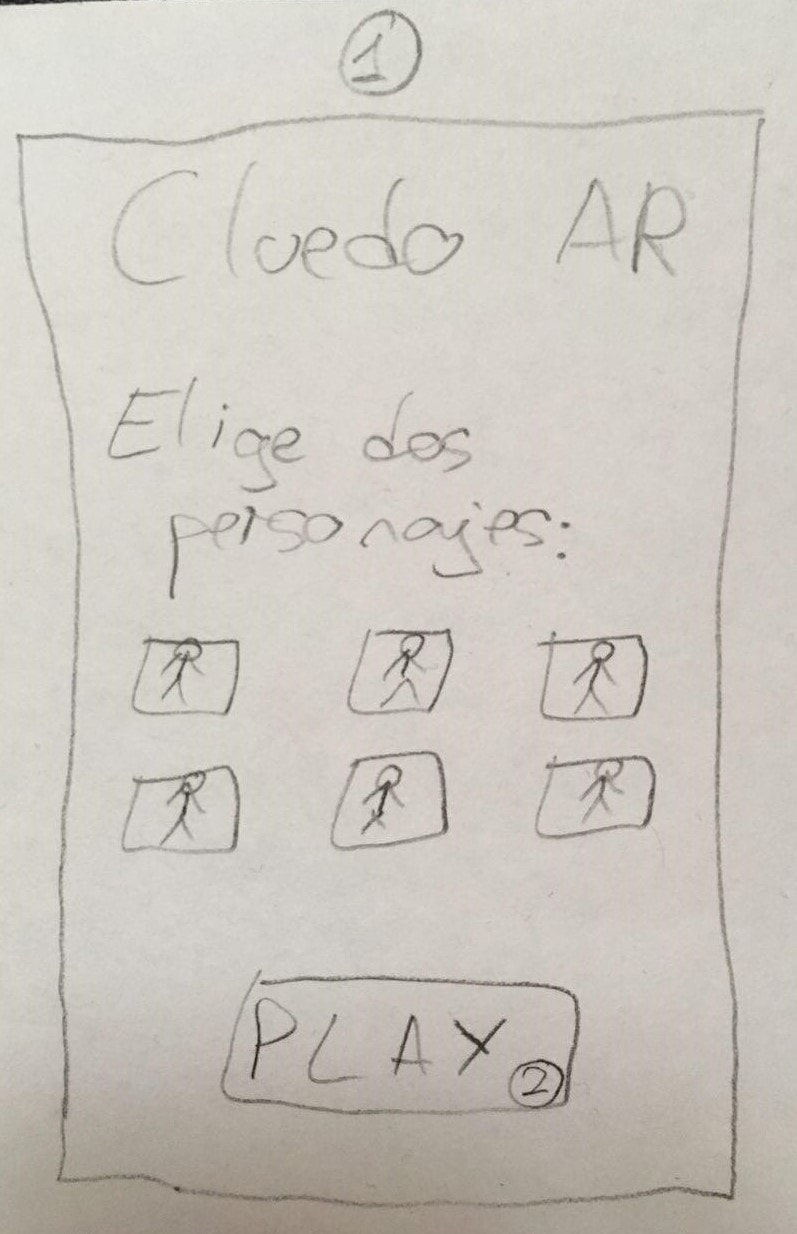
\includegraphics[height=3.5in]{b1.jpg}}
  \qquad
  \subfigure{
  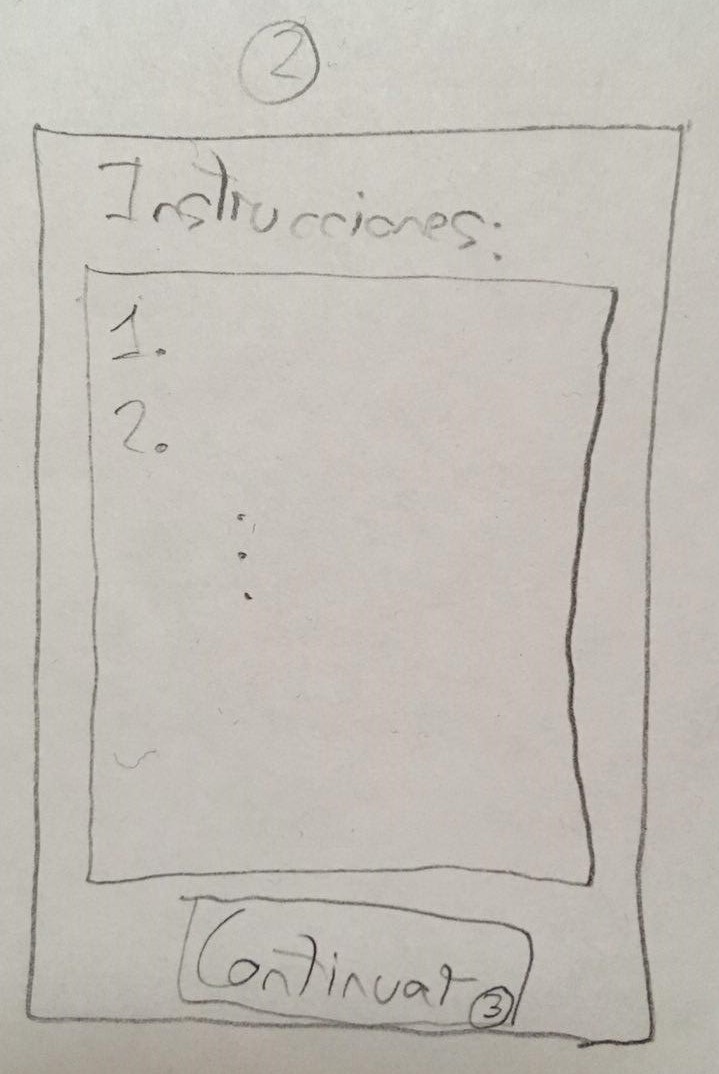
\includegraphics[height=3.5in]{b2.jpg}}
\end{figure}

\newpage

Bocetos sobre la pantalla de juego, con diferentes visualizaciones:

\begin{figure}[h]
  \subfigure{
  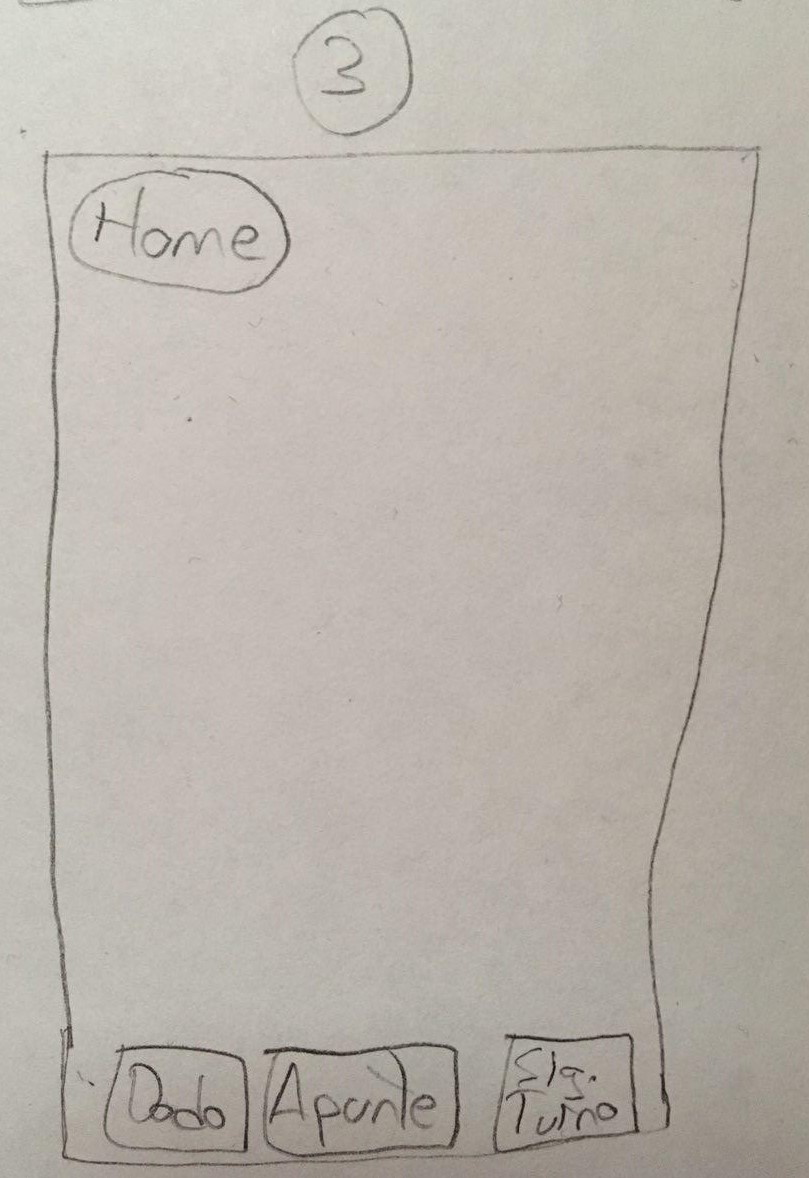
\includegraphics[height=3.05in]{b3.jpg}}
  \qquad
  \subfigure{
  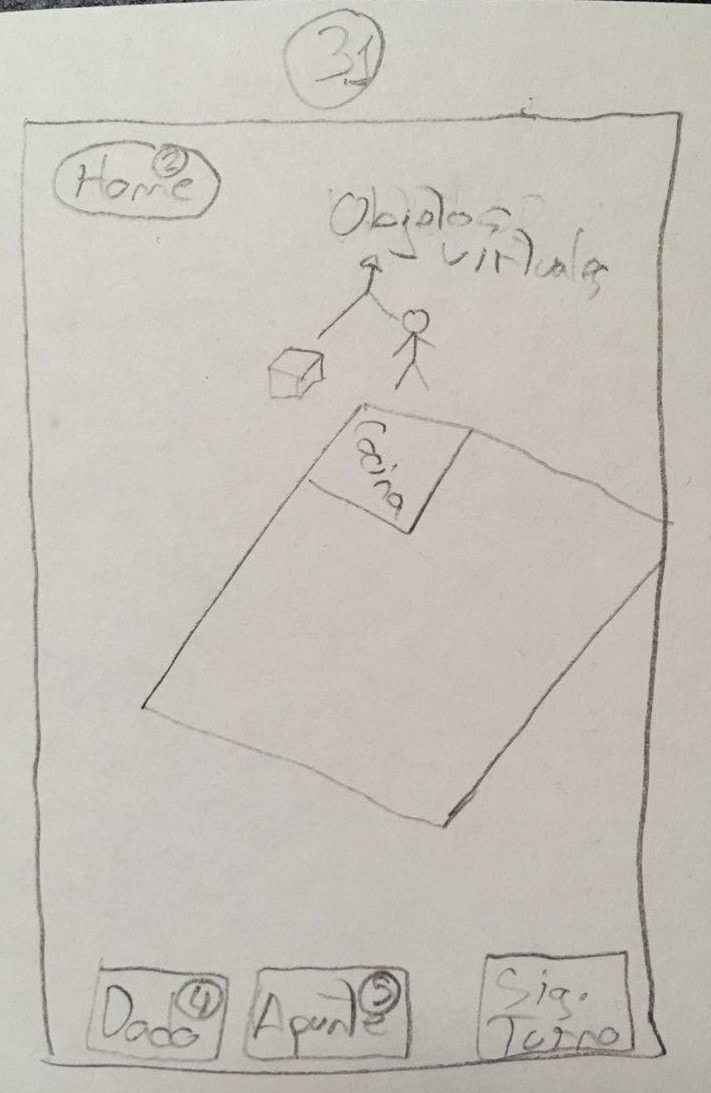
\includegraphics[height=3.1in]{b3-1.jpg}}
\end{figure}

Bocetos sobre la pantalla de juego, y la de selección de habitación:

\begin{figure}[h]
  \centering
  \subfigure{
  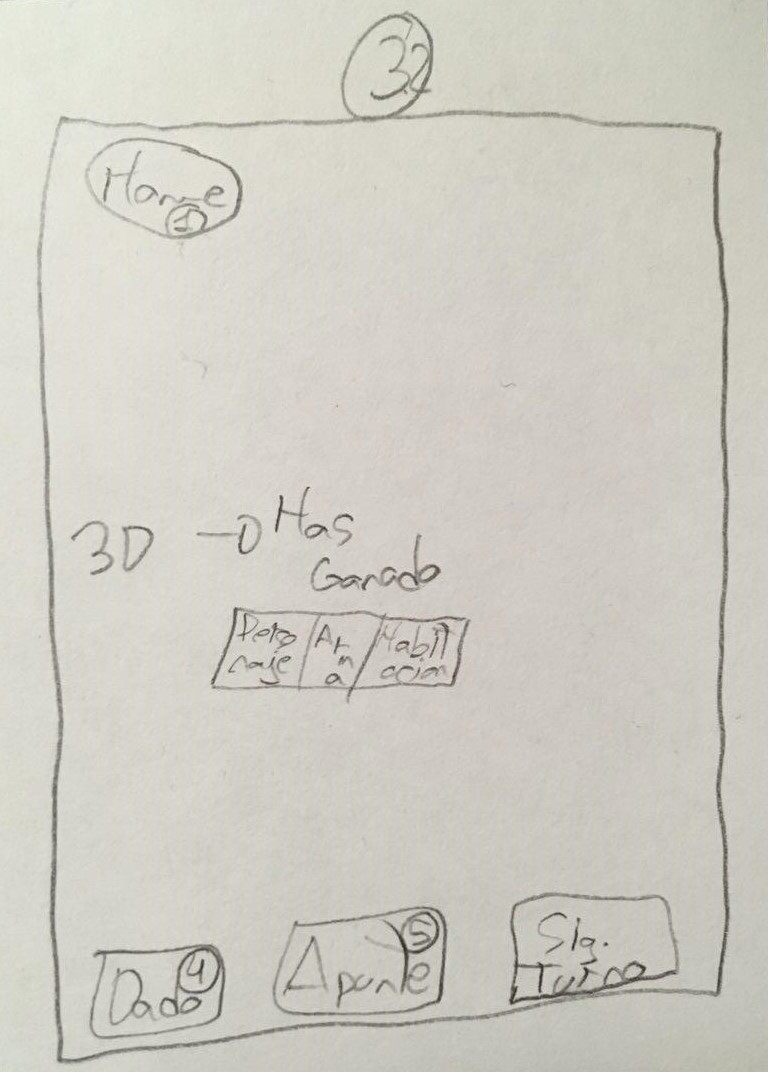
\includegraphics[height=2.95in]{b3-2.jpg}}
  \qquad
  \subfigure{
  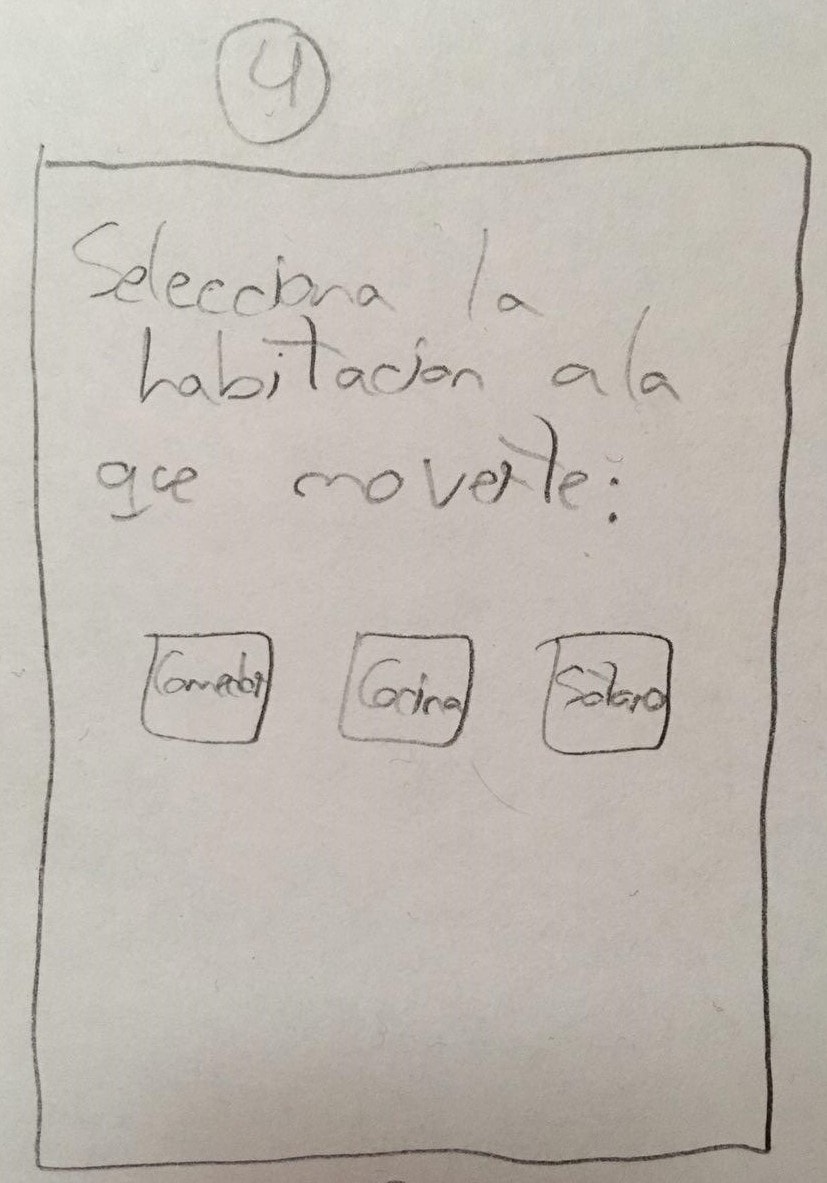
\includegraphics[height=2.95in]{b4.jpg}}
\end{figure}

\newpage

Bocetos sobre la pantalla de tomar apuntes y la pantalla cuando un jugador gana el juego:

\begin{figure}[h]
  \centering
  \subfigure{
  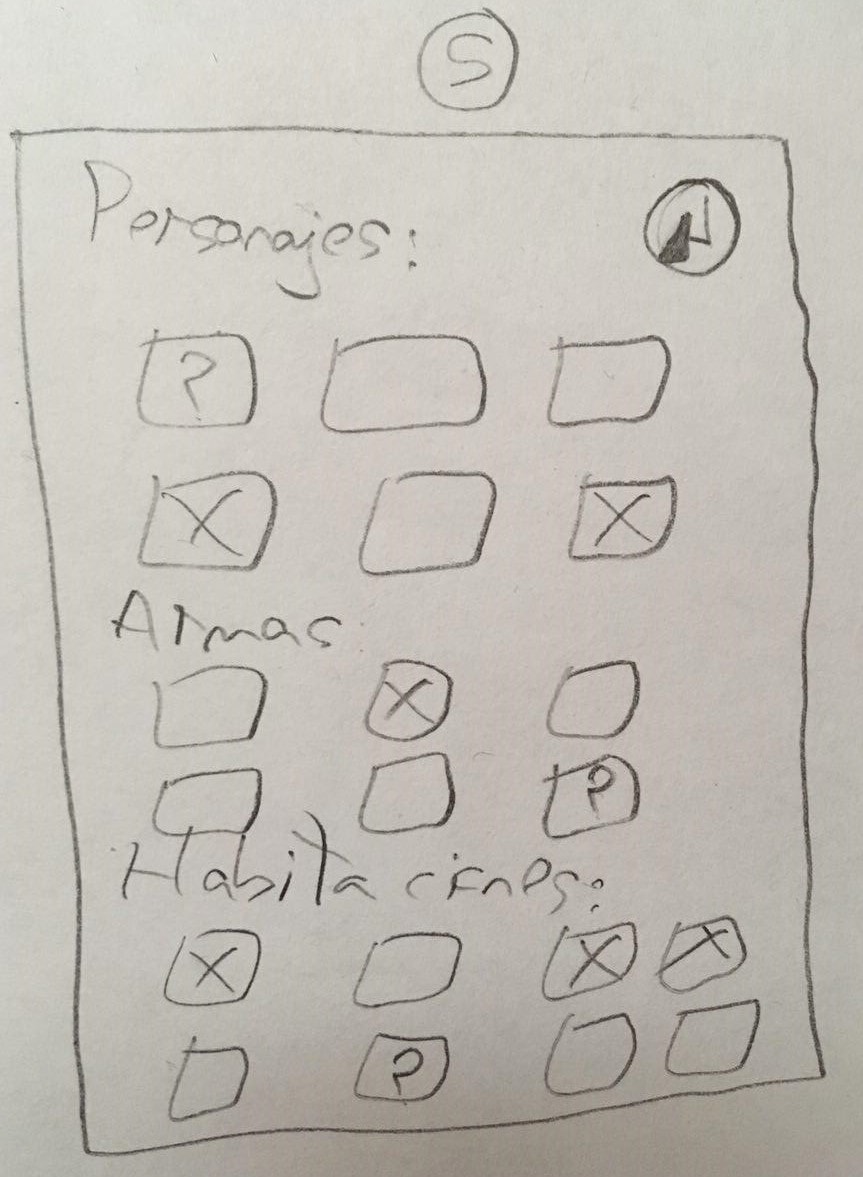
\includegraphics[height=3in]{b5.jpg}}
  \qquad
  \subfigure{
  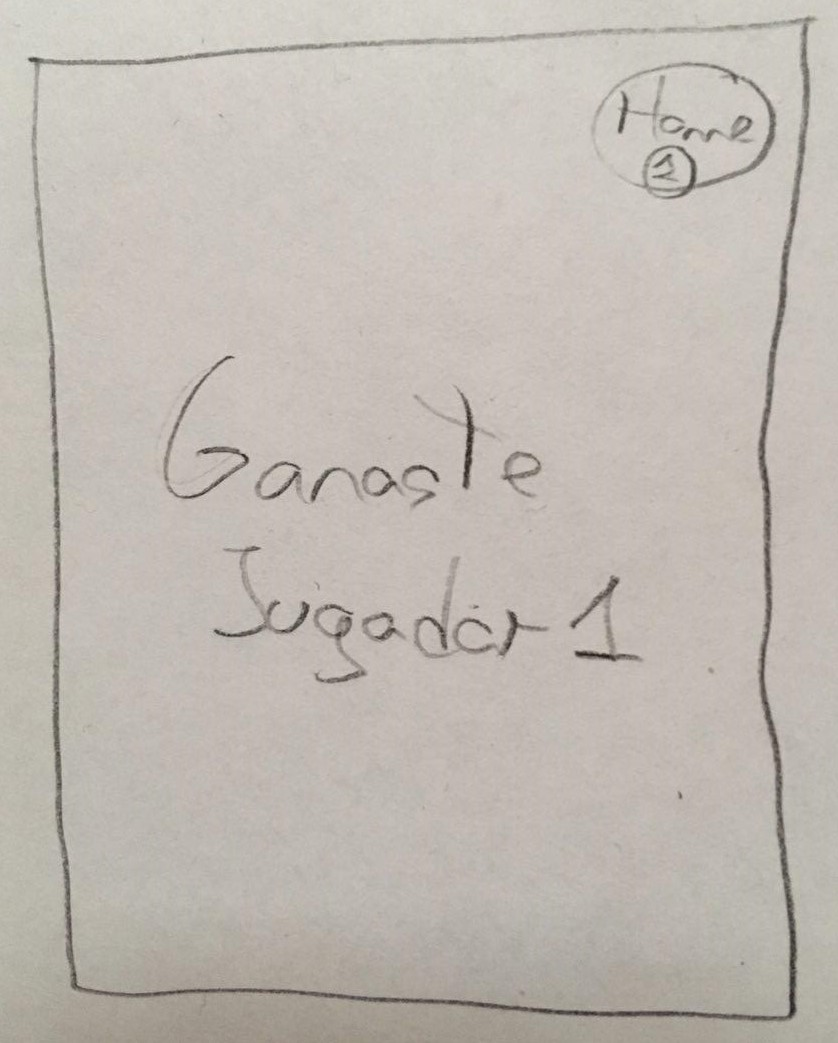
\includegraphics[height=3in]{b6.jpg}}
\end{figure}


\section{Tablas de usabilidad para los bocetos} \label{tablas-usabilidad-bocetos}

\begin{table}
  \begin{center}
    \begin{tabular}{|p{2.5cm}|p{1.75cm}|p{1.25cm}|p{1.25cm}|p{2.75cm}|p{3.5cm}|}

      \hline
        \rowcolor{Gray} \textbf{Escenario de uso}
        & \textbf{Tarea}
        & \textbf{Éxito/ Fracaso}
        & \textbf{Tiempo}
        & \textbf{Dificultades encontradas}
        & \textbf{Comentarios}\\

      \hline
      El usuario se encuentra jugando una partida
      & Seleccionar ajustes iniciales
      & Éxito
      & 10 seg
      & Le cuesta seleccionar el personaje con el dedo
      & Hacer los botones de personaje mas grandes para facilitar a los usuarios este proceso\\

      \hline
      El usuario se encuentra jugando una partida
      & Comenzar el juego
      & Éxito
      & 5 seg
      & Ninguna
      &\\

      \hline
      El usuario se encuentra jugando una partida
      & Salir de las instrucciones
      & Éxito
      & 5 seg
      & Ninguna
      &\\

      \hline
      El usuario se encuentra jugando una partida
      & Escanear el tablero
      & Éxito
      & 10 seg
      & Ninguna
      &\\

      \hline
      El usuario se encuentra jugando una partida
      & Lanzar el dado
      & Éxito
      & 20 seg
      & Ninguna
      & Añadir imagen con el nombre de la habitación para facilitar a los usuarios este proceso\\

      \hline
      El usuario se encuentra jugando una partida
      & Hacer apunte
      & Éxito
      & 25 seg
      & Ninguna
      &\\

      \hline
      El usuario se encuentra jugando una partida
      & Escanear acusación
      & Éxito
      & 20 seg
      & Ninguna
      &\\

      \hline
      El usuario se encuentra jugando una partida
      & Pasar de turno
      & Éxito
      & 5 seg
      & Ninguna
      &\\

      \hline
      El usuario se encuentra jugando una partida
      & Volver a la pantalla inicial
      & Fracaso
      & 15 seg
      & No sabe donde seleccionar terminar partida
      & Cambiar el texto del botón home por Terminar partida\\

      \hline
      El usuario se encuentra jugando una partida
      & Finalizar después de ganar
      & Éxito
      & 5 seg
      & No sabe donde seleccionar para salir de esa pantalla
      & Cambiar el texto del botón home por Continuar\\

      \hline

    \end{tabular}

    \caption{Resultados usabilidad con Usuario 1.}
    \label{tabla-bocetos-usuario1}

  \end{center}
\end{table}


\begin{table}
  \begin{center}
    \begin{tabular}{|p{2.5cm}|p{1.75cm}|p{1.25cm}|p{1.25cm}|p{2.75cm}|p{3.5cm}|}

      \hline
        \rowcolor{Gray} \textbf{Escenario de uso}
        & \textbf{Tarea}
        & \textbf{Éxito/ Fracaso}
        & \textbf{Tiempo}
        & \textbf{Dificultades encontradas}
        & \textbf{Comentarios}\\

      \hline
      El usuario se encuentra jugando una partida
      & Seleccionar ajustes iniciales
      & Éxito
      & 5 seg
      & Ninguna
      &\\

      \hline
      El usuario se encuentra jugando una partida
      & Comenzar el juego
      & Éxito
      & 5 seg
      & Ninguna
      &\\

      \hline
      El usuario se encuentra jugando una partida
      & Salir de las instrucciones
      & Éxito
      & 5 seg
      & Ninguna
      &\\

      \hline
      El usuario se encuentra jugando una partida
      & Escanear el tablero
      & Éxito
      & 15 seg
      & Ninguna
      &\\

      \hline
      El usuario se encuentra jugando una partida
      & Lanzar el dado
      & Éxito
      & 10 seg
      & Ninguna
      & \\

      \hline
      El usuario se encuentra jugando una partida
      & Hacer apunte
      & Fracaso
      & 25 seg
      & No comprendía el funcionamiento de cómo realizar un apunte
      & Explicar en la pantalla de instrucciones inicial como se realiza un apunte\\

      \hline
      El usuario se encuentra jugando una partida
      & Escanear acusación
      & Éxito
      & 10 seg
      & Ninguna
      &\\

      \hline
      El usuario se encuentra jugando una partida
      & Pasar de turno
      & Éxito
      & 3 seg
      & Ninguna
      &\\

      \hline
      El usuario se encuentra jugando una partida
      & Volver a la pantalla inicial
      & Fracaso
      & 7 seg
      & No encontraba el botón de inicio
      & Cambiar el texto del botón a español y mas grande\\

      \hline
      El usuario se encuentra jugando una partida
      & Finalizar después de ganar
      & Éxito
      & 3 seg
      & No sabe que significa home, el botón es pequeño y poco accesible
      & Cambiar el texto del botón a español y mas grande\\

      \hline

    \end{tabular}

    \caption{Resultados usabilidad con Usuario 2.}
    \label{tabla-bocetos-usuario2}

  \end{center}
\end{table}


\begin{table}
  \begin{center}
    \begin{tabular}{|p{2.5cm}|p{1.75cm}|p{1.25cm}|p{1.25cm}|p{2.75cm}|p{3.5cm}|}

      \hline
        \rowcolor{Gray} \textbf{Escenario de uso}
        & \textbf{Tarea}
        & \textbf{Éxito/ Fracaso}
        & \textbf{Tiempo}
        & \textbf{Dificultades encontradas}
        & \textbf{Comentarios}\\

      \hline
      El usuario se encuentra jugando una partida
      & Seleccionar ajustes iniciales
      & Éxito
      & 5 seg
      & Ninguna
      & Activar el botón de play cuando haya seleccionado 2 personajes\\

      \hline
      El usuario se encuentra jugando una partida
      & Comenzar el juego
      & Éxito
      & 5 seg
      & Ninguna
      &\\

      \hline
      El usuario se encuentra jugando una partida
      & Salir de las instrucciones
      & Éxito
      & 5 seg
      & Ninguna
      &\\

      \hline
      El usuario se encuentra jugando una partida
      & Escanear el tablero
      & Éxito
      & 3 seg
      & Ninguna
      &\\

      \hline
      El usuario se encuentra jugando una partida
      & Lanzar el dado
      & Éxito
      & 15 seg
      & El botón de dado no era muy descriptivo y el usuario no sabia si ahí se lanzaba
      & Cambiar el texto del botón dado a Lanzar dado\\

      \hline
      El usuario se encuentra jugando una partida
      & Hacer apunte
      & Éxito
      & 20 seg
      & El botón usuario no entiende que pasa al pulsar el botón de apunte
      & Cambiar el texto del botón de apunte a Notas\\

      \hline
      El usuario se encuentra jugando una partida
      & Escanear acusación
      & Éxito
      & 10 seg
      & Ninguna
      &\\

      \hline
      El usuario se encuentra jugando una partida
      & Pasar de turno
      & Éxito
      & 3 seg
      & Ninguna
      &\\

      \hline
      El usuario se encuentra jugando una partida
      & Volver a la pantalla inicial
      & Éxito
      & 3 seg
      & Ninguna
      &\\

      \hline
      El usuario se encuentra jugando una partida
      & Finalizar después de ganar
      & Éxito
      & 3 seg
      & Ninguna
      & Camiar el texto a Continuar y cambiar su posición y tamaño\\

      \hline

    \end{tabular}

    \caption{Resultados usabilidad con Usuario 3.}
    \label{tabla-bocetos-usuario3}

  \end{center}
\end{table}

\end{itemize}
